\documentclass[a4paper, 12pt]{article}
\usepackage{blindtext}
\usepackage[margin=2 cm]{geometry}
\usepackage[spanish]{babel}
\usepackage[utf8]{inputenc}
\usepackage{array}
\usepackage{amsmath}
\usepackage{graphicx}
\usepackage{ifthen}
\usepackage{commath}
\usepackage{esint}
\usepackage{mathtools}
\usepackage{listing}
\usepackage{multirow}
\usepackage{tabto}
\usepackage[backend=biber]{biblatex}
\usepackage{csquotes}
\usepackage{float}
\usepackage{amssymb}
\usepackage{physics}
\usepackage{hyperref}
\usepackage[shortlabels]{enumitem}
\selectlanguage{spanish}
\decimalpoint

\begin{document}
    \begin{center}
        \begin{Large}

            \begin{figure}[H]	
                \centering
                
\includegraphics[width = 6cm]{./img/logo_UADY.png}
                \label{uady}
            \end{figure}
            \textsc{FACULTAD DE INGENIERÍA}
                
            \medskip

            Curso Agosto - Diciembre 2021

            \medskip

            \textsc{Física Computacional}

            \medskip

            \textsl{Actividad de Aprendizaje 4}

            \medskip

            Br. Alejandro Santoscoy Rivero

            \medskip

            Dr. Francisco Ramón Peñuñuri Anguiano

            \rule{0.3\paperwidth}{0.5pt}

            \medskip

            9 de Diciembre de 2021

        \end{Large}
    \end{center}
    \pagenumbering{roman}
    \newpage
    \pagenumbering{arabic}

    \section{Problema}

    1. Grafique $y(x)$ para las siguientes ecuaciones diferenciales

    \begin{enumerate}[a)]
        \item $y''(x) + \sin (xy'y)+2x = 5; y(0) = 1, y'(0) = 2$ para $x \in [0,3]$
        \item $y^{(4)}+\sin xy^{(3)} + \exp (-x) y'' + y' - xy = 0$ con el vector de condiciones iniciales $Y_0 = [1,2,3,4]$, para $x \in [1,2]$ (Observe que $X_0 = 1$)
    \end{enumerate}

    Estos ejerciciso se resuelven con el método de Runge Kuta de 4to orden.

    Lo primero que se hace es definir la función en general en Octave.

    \begin{verbatim}
        function local = RK4(fun_rhs,a,b,init_cond,n_ints)
  
        nrow = n_ints+1;
        ncol = size(init_cond)(2);
        
        local = zeros(nrow,ncol);
        
        h = (b - a)/n_ints;
        
        x = zeros(nrow,1);
        y = zeros(nrow,ncol);
        x(1) = a;
        y(1,:) = init_cond;
        
        for ii=1:n_ints
            K1 = h*fun_rhs(x(ii),y(ii,:));
            K2 = h*fun_rhs(x(ii)+0.5*h, y(ii,:)+0.5*K1);
            K3 = h*fun_rhs(x(ii)+0.5*h, y(ii,:)+0.5*K2);
            K4 = h*fun_rhs(x(ii)+h, y(ii,:)+K3);
            
            x(ii+1) = x(ii) + h;
            y(ii+1,:) = y(ii,:) + (1/6)*(K1 + 2*K2 + 2*K3 + K4);
        end
        
        local = cat(2, x, y);
        end
    \end{verbatim}

    Una vez definida la función ahora es resolver cada ecuación diferencial para obtener las funciones derivadas de ellas.

    \begin{enumerate}[a)]
        \item Se está tratando de una ecuación diferencial de 2do orden, así que tenemos 2 condiciones de frontera.
        
        Primero se realiza un cambio de variable dependiente:

        \begin{align*}
            u_1 &= y \\
            u_2 &= y'
        \end{align*}

        Entonces la ecuación difetencial de puede reescribir como

        \[
            u_2'+ \sin (x u_1 u_2) + 2x = 5
        \]

        Despejando $u_2'$

        \[
            u_2' = 5 - 2x - \sin (x u_1 u_2)
        \]

        Y por reglas de igualdad, podemos decir que $u_1' = u_2$

        Teniendo estas dos funciones derivadas y las condiciones de frontera, entonces ya se puede codificar el comportamiento como

        \begin{verbatim}
            fr = @(x,y) [y(2), 5-2*x-sin(x*y(1)*y(2))]

            a=0;
            b=2;
            y0=[1,2];
            npts = 500;
            sol = RK4(fr,a,b,y0,npts);


            hold on;
            scatter(sol(:,1),sol(:,2),3,'filled');
        \end{verbatim}

        El resultado de los puntos obtenidos es la siguiente:

        \begin{figure}[ht!]
            \centering
            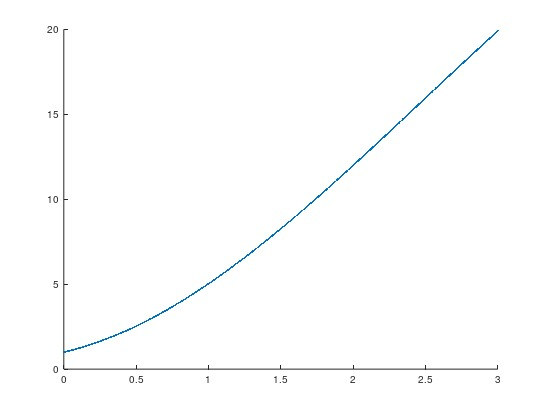
\includegraphics[width=8cm]{img/e1a.jpeg}
        \end{figure}

        \item Para la siguiente ecuación, la cual es de 4to orden, se realiza un procedimiento similar
        
        \begin{align*}
            u_1 &= y \\
            u_2 &= y' \\
            u_3 &= y'' \\
            u_4 &= y''' \\
        \end{align*}

        Entonces la ecuación se puede reescribir como

        \[
            u_4' = xu_1 - u_2 - \exp(-x)u_3 - \sin(xu_4)
        \]

        Al escribir las funciones derivadas y las condiciones iniciales:

        \begin{verbatim}
            fr = @(x,y) [y(2),y(3),y(4),x*y(1)-y(2)-exp(-x)*y(3)
            -sin(x*y(4))]

            a=0;
            b=2;
            y0=[1,2,3,4];
            npts = 500;
            sol = RK4(fr,a,b,y0,npts);

            hold on;
            scatter(sol(:,1),sol(:,2),3,'filled');
        \end{verbatim}

        Y la gráfica queda de la siguiente manera

        \begin{figure}[ht!]
            \centering
            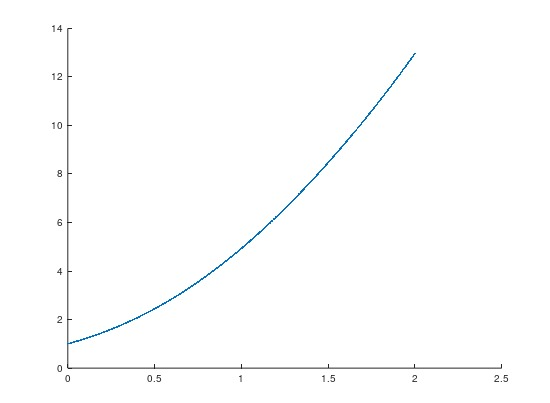
\includegraphics[width=8cm]{img/e1b.jpeg}
        \end{figure}

    \end{enumerate}

    2. La ecuación de movimiento para un péndulo amoritugado es:

    \[
        \ddot{\theta} + \frac{c}{m} \dot{\theta} + \frac{g}{l} \sin \theta = 0  
    \]

    Tomando $m=1 kg$, $l=1m$, $g=9.8m/s^2$ y $c=0.5 Ns/m$ 7 las condiciones iniciales son $\theta(0) = \pi/2 y \dot{\theta}(0) = 0$. Haga una gráfica de la tensión en la cuerda como función del tiempo.

    Se realiza una sustitución de variables

    \[
        \omega = \dot(\theta)
    \]

    Reesbribiendo la función derivada

    \[
        \dot{\omega} = -\frac{c}{m}\omega - \frac{g}{l} \sin \theta
    \]

    Pasando a código:

    \begin{verbatim}
        c = 0.5;
        g = 9.8;
        l = 1;
        m = 1;

        fr = @(x,y) [y(2), -(c/m)*y(2)- (g/l)*sin(y(1))];

        a=0;
        b=10;
        y0=[pi/2,2];
        npts = 1000;
        sol = RK4(fr,a,b,y0,npts);


        hold on;
        scatter(sol(:,1),sol(:,2),3,'filled');
    \end{verbatim}

    Y la gráfica que se obtiene es la siguiente

    \begin{figure}[ht!]
        \centering
        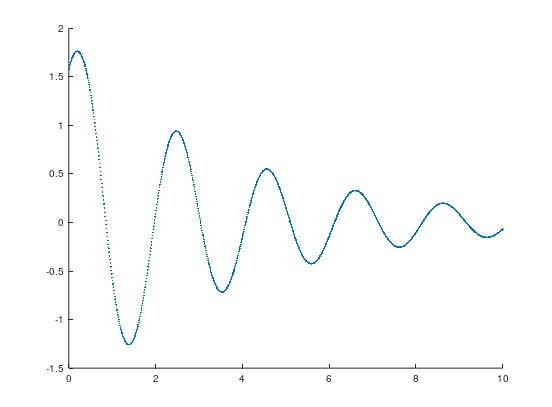
\includegraphics[width=8cm]{img/e2.jpeg}
    \end{figure}

    Se puede observar el claro comportamiento oscilatorio.


    Entonces

    3. Reproduzca la figura 5.b ($u_1(t) = u_2(t) = 0$) de la referencia [1]

    4. Implemente los número duales y sobrecargue las siguientes funciones y operadores.

    \verb|(\^), (*), (+), (-), (/), (==), (!=), acos, acosh, asin, asinh, atan,|
    
    \verb|atan2, atanh, sin, cos, cosh, erf, sinh, tan, tanh, exp, log,|
    
    \verb|sqrt, abs|.

    5. Usando las funciones del ejercicio anterior, implemente $\nabla f(x0)$ y $Jf(x0)$; una función que permita calcular el gradiente y otra que calcule el Jacobiano de una función evaluada en el punto $x_0$.
    


\end{document}